\chapter{Auswertung}
\label{kap:auswertung}

Dieses Kapitel beantwortet drei Fragen: Was leistet die Pipeline auf echten Daten
(Abschnitte~\ref{sec:metriken}--\ref{sec:simtoreal})? Welche Parameter dominieren
das Ergebnis (Abschnitte~\ref{sec:imgsz} und \ref{sec:infparam})? Und trägt die
aufwendigste Augmentierungsentscheidung -- die physikalisch motivierte Verdeckung
-- ihren Aufwand (Abschnitt~\ref{sec:ablation})?

\section{Bewertungsprotokoll und Metriken}
\label{sec:metriken}

\subsection{Die verwendeten Metriken in Worten}

Damit die folgenden Zahlen lesbar sind, seien die Metriken zunächst knapp und
anschaulich erklärt. Eine Detektion gilt als Treffer (\emph{True Positive}, TP),
wenn ihre Box eine Ground-Truth-Box mit einer Überlappung von mindestens $t$
umschließt; die Überlappung wird als \emph{Intersection over Union} gemessen:
\begin{equation}
\mathrm{IoU}(A, B) = \frac{|A \cap B|}{|A \cup B|}.
\end{equation}
Jede Ground-Truth-Box kann höchstens einmal getroffen werden; überzählige
Detektionen sind Falsch-Positive (FP), nicht getroffene Ground-Truth-Boxen sind
Falsch-Negative (FN). Daraus folgen:

\begin{description}[leftmargin=4.6em,style=sameline,font=\normalfont\itshape]
  \item[Precision] $P = \mathrm{TP}/(\mathrm{TP}+\mathrm{FP})$ -- der Anteil der
  Detektionen, die richtig sind. Wenig FP bedeutet hohe Precision.
  \item[Recall] $R = \mathrm{TP}/(\mathrm{TP}+\mathrm{FN})$ -- der Anteil der
  vorhandenen Objekte, die gefunden wurden.
  \item[F1] das harmonische Mittel $2PR/(P+R)$. Berichtet wird das \emph{beste}
  F1 über alle Konfidenzschwellen sowie die zugehörige Schwelle $c^*$; das ist
  der Betriebspunkt, den man in einer Anwendung wählen würde.
  \item[AP / mAP] die Fläche unter der Precision-Recall-Kurve
  \parencite{everingham2010}. \mAPfifty{} verwendet $t = 0{,}5$, \mAPseven{}
  $t=0{,}75$, \mAPall{} den Mittelwert über $t = 0{,}50; 0{,}55; \dots; 0{,}95$
  nach COCO-Konvention \parencite{lin2014coco}. Da hier nur eine Klasse existiert,
  ist mAP mit AP identisch.
  \item[Zählfehler] die für die Anwendung eigentlich relevante Größe: die
  Differenz zwischen der Anzahl der Detektionen am Betriebspunkt $c^*$ und der
  Anzahl der Ground-Truth-Objekte.
\end{description}

Zwei Lesehinweise sind wichtig. Erstens sagt ein hoher \mAPfifty{}-Wert bei
gleichzeitig niedrigem \mAPseven{}-Wert, dass die Objekte \emph{gefunden}, aber
nicht präzise \emph{lokalisiert} werden -- bei 20\px{} großen Objekten ist das
nach Gleichung~\eqref{eq:ioushift} zu erwarten. Zweitens ist der Zählfehler nicht
aus mAP ableitbar: Er hängt zusätzlich davon ab, ob sich FP und FN gegenseitig
kompensieren.

\subsection{Eigenes Bewertungsframework und seine Verifikation}

Die Bewertung erfolgt über eine eigene Implementierung
(\code{src/evaluate.py}) und nicht über die Bewertungsfunktion der
Werkzeugkette. Der Grund ist, dass Zählfehler, mittlere Treffer-IoU und der
F1-optimale Betriebspunkt gebraucht werden -- Größen, die die Standardfunktion
nicht ausgibt -- und dass die Zuordnungslogik nachvollziehbar sein muss.

Eine eigene Metrikimplementierung ist allerdings eine Fehlerquelle. Sie wird
deshalb gegen die Referenzimplementierung geprüft
(Tabelle~\ref{tab:crosscheck}).

\begin{table}[htbp]
\centering
\caption[Verifikation der Metrikimplementierung]{Verifikation der eigenen
Metrikimplementierung gegen die Referenzimplementierung der Werkzeugkette,
nativer Maßstab.}
\label{tab:crosscheck}
\small
\begin{tabular}{@{}lcc@{}}
\toprule
 & \textbf{eigene Implementierung} & \textbf{Referenz} \\
\midrule
\code{val} \mAPfifty{} / \mAPall{}  & 0{,}886 / 0{,}597 & 0{,}897 / 0{,}599 \\
\code{test} \mAPfifty{} / \mAPall{} & 0{,}888 / 0{,}437 & 0{,}891 / 0{,}424 \\
\bottomrule
\end{tabular}
\end{table}

Die Abweichung liegt bei maximal 1,3\PP{} und ist durch Detailunterschiede in
der AP-Interpolation und der Zuordnungsreihenfolge erklärbar. Die eigene
Implementierung ist damit verifiziert; alle folgenden Zahlen stammen aus ihr,
sodass sie untereinander vergleichbar sind.

\section{Hauptergebnis}
\label{sec:hauptergebnis}

\begin{table}[htbp]
\centering
\caption[Hauptergebnis]{Ergebnis des besten Modells bei nativem Maßstab.
$c^*$ ist die F1-optimale Konfidenzschwelle, \enquote{mittl.\ IoU} die mittlere
Überlappung der Treffer.}
\label{tab:hauptergebnis}
\footnotesize
\resizebox{\textwidth}{!}{%
\begin{tabular}{@{}lrrrrrrrrr@{}}
\toprule
\textbf{Split} & \mAPfifty{} & \mAPseven{} & \mAPall{} & \textbf{bestes F1} &
$c^*$ & $P$ & $R$ & \textbf{mittl.\ IoU} & \textbf{Zählung} \\
\midrule
\code{val} (real)  & 0{,}886 & 0{,}793 & 0{,}597 & 0{,}862 & 0{,}336 & 0{,}872 & 0{,}852 & 0{,}824 & 86/88 \\
\code{test} (real) & 0{,}888 & 0{,}320 & 0{,}437 & 0{,}894 & 0{,}263 & 0{,}905 & 0{,}884 & 0{,}748 & 84/86 \\
\code{sval} (synth.) & 0{,}982 & 0{,}935 & 0{,}828 & 0{,}964 & 0{,}450 & 0{,}972 & 0{,}956 & 0{,}899 & 7128/7248 \\
\bottomrule
\end{tabular}}
\end{table}

\absatz{Wie ist das zu lesen?} Ein ausschließlich auf synthetischen Bildern
trainiertes Modell findet auf echten, nie im Training gesehenen Aufnahmen etwa
88--89\,\% der Objekte bei vergleichbarer Precision. Für die eigentliche
Anwendung ist der Zählfehler die relevante Größe: 86 statt 88 und 84 statt 86
Objekte, also \textbf{2,3\,\% Zählfehler} auf beiden realen Aufnahmen. Bei der
auf \code{val} gewählten Inferenzauflösung (Abschnitt~\ref{sec:imgsz}) steigt
\mAPfifty{} auf \code{test} auf 0,928, mit Test-Time-Augmentation auf 0,934.

\absatz{Der auffällige Unterschied zwischen den Splits.} \code{val} erreicht
\mAPseven{} = 0,793, \code{test} nur 0,320 -- bei praktisch identischem
\mAPfifty{}. Das ist kein Widerspruch, sondern der in
Abschnitt~\ref{sec:ioukleinobjekt} vorhergesagte Effekt: Die Objekte in
\code{test} sind kleiner (Median 19,6\px{} gegen 27,4\px{}). Nach
Gleichung~\eqref{eq:ioushift} kostet bei einem 20\px{}-Objekt ein Boxfehler von
2\px{} bereits 0,18 IoU. Die mittlere Treffer-IoU bestätigt das direkt: 0,824 auf
\code{val}, 0,748 auf \code{test}.

Die Objektgröße ist allerdings nur ein Teil der Erklärung. Den größeren Teil
liefert ein \emph{systematischer Größenversatz zwischen Generatorlabel und
Handannotation}, der in Abschnitt~\ref{sec:boxversatz} aufgeschlüsselt wird: Auf
\code{test} sind die vorhergesagten Boxen im Median 11,6\,\% kleiner als die
annotierten, auf \code{val} nur 3,9\,\%. Eine Sensitivitätsrechnung, die diesen
Versatz herausrechnet, hebt \mAPseven{} auf \code{test} von 0,320 auf 0,714.
\mAPall{} ist bei dieser Objektgröße folglich weniger ein Maß für die
Detektionsqualität als für Pixelauflösung und Labelkonvention -- eine
Feststellung, die für die Interpretation aller folgenden Tabellen gilt.

\begin{figure}[htbp]
\centering
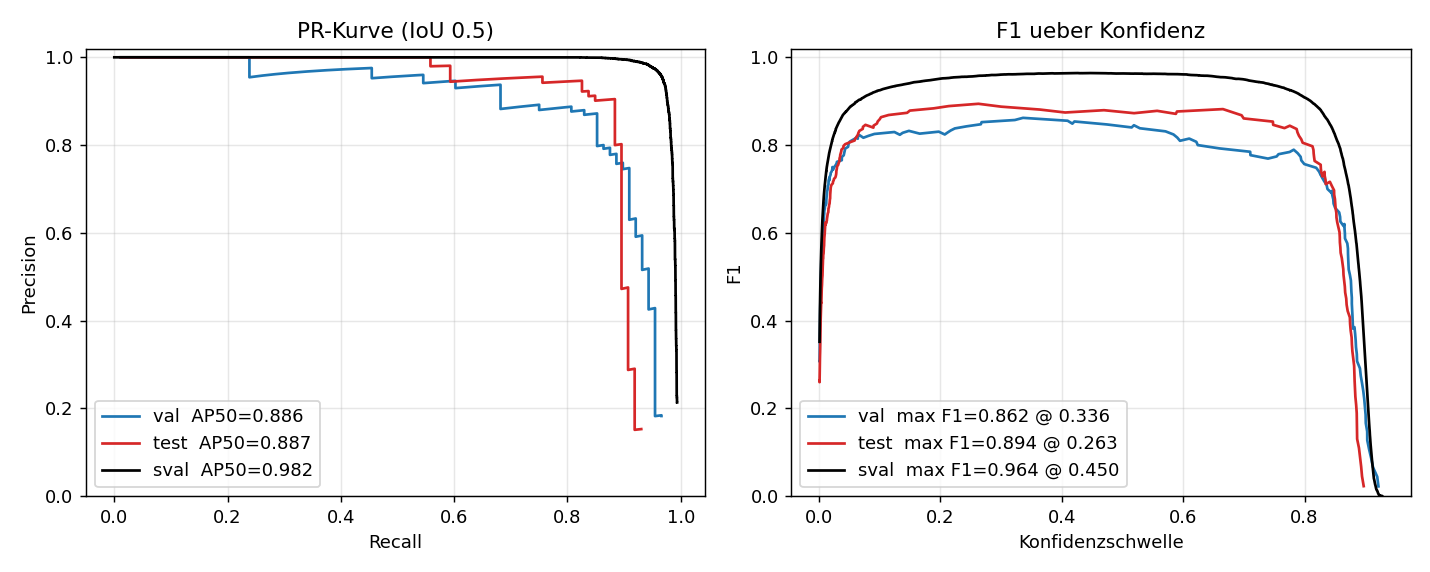
\includegraphics[width=\textwidth]{abbildungen/pr_kurven.png}
\caption[Precision-Recall-Kurven]{Precision-Recall-Kurven der drei Splits. Der
Abstand zwischen der synthetischen Kurve (\code{sval}) und den beiden realen
Kurven ist der Sim-to-Real-Abstand aus Abschnitt~\ref{sec:simtoreal}.}
\label{abb:prkurven}
\end{figure}

\begin{figure}[htbp]
\centering
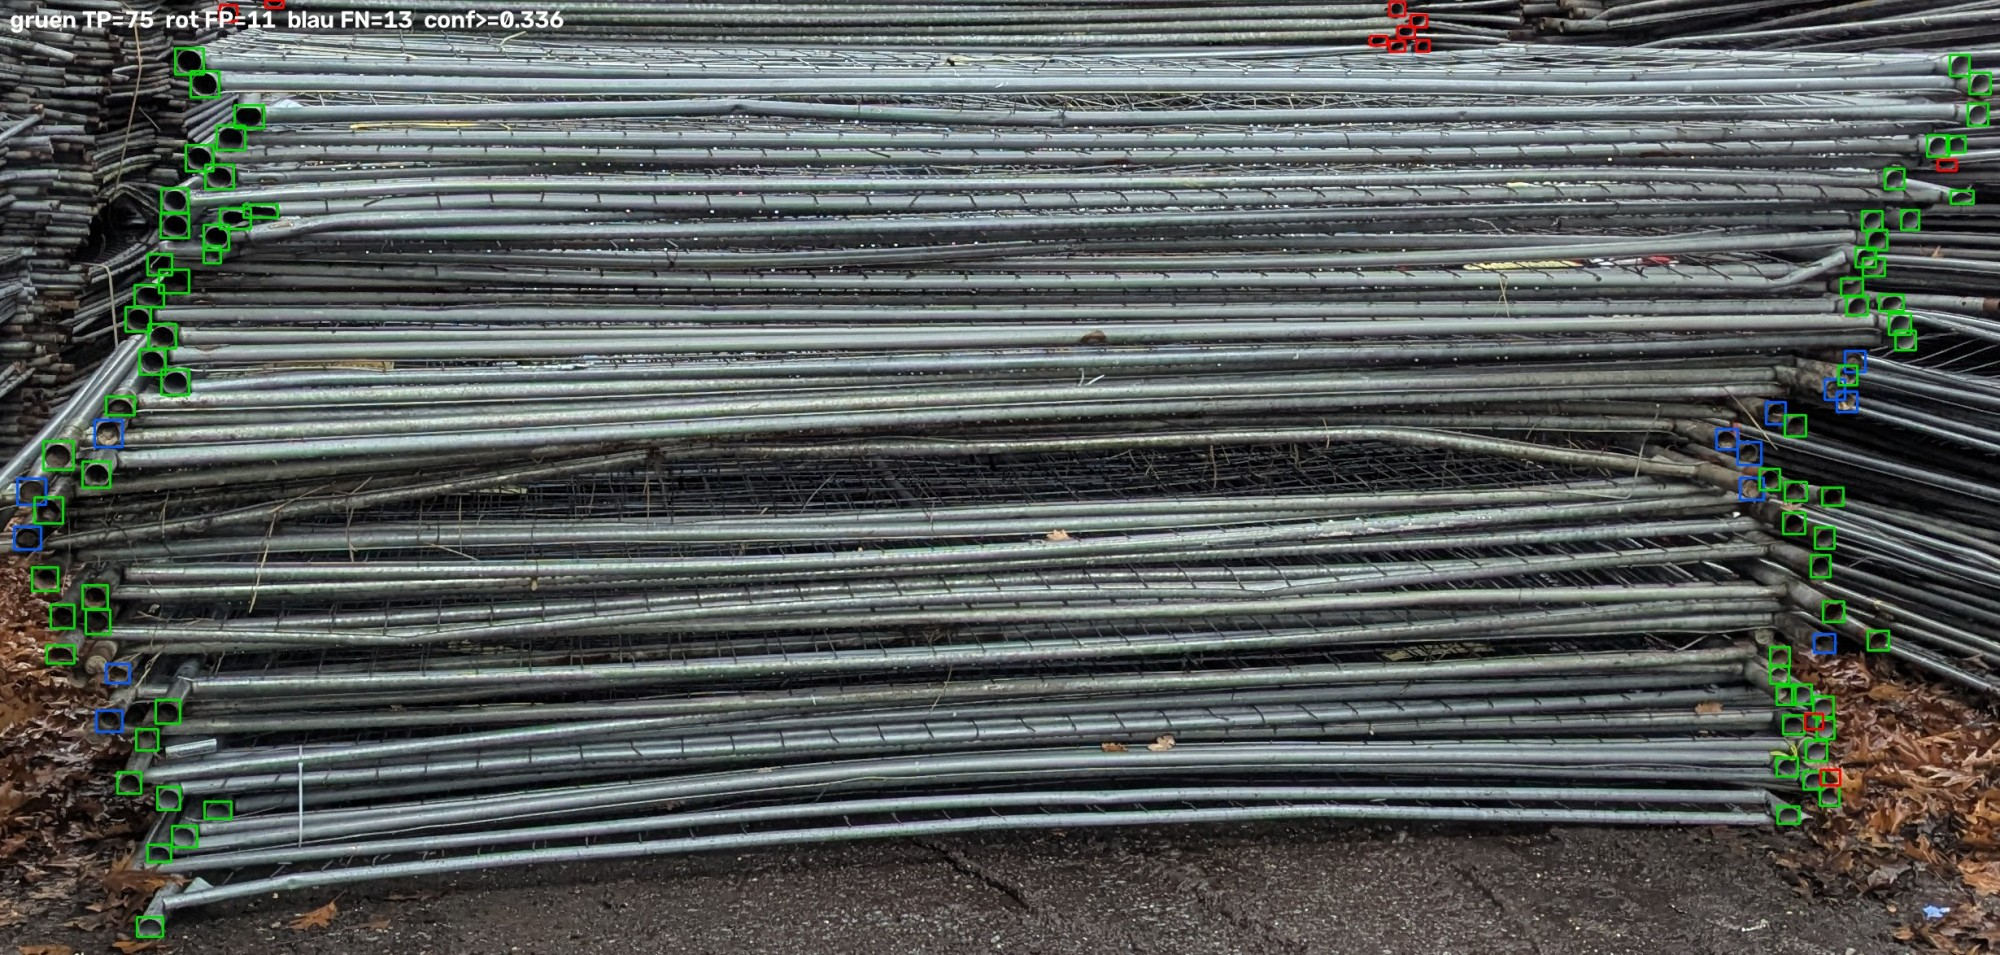
\includegraphics[width=\textwidth]{abbildungen/qual_val.jpg}

\vspace{2mm}
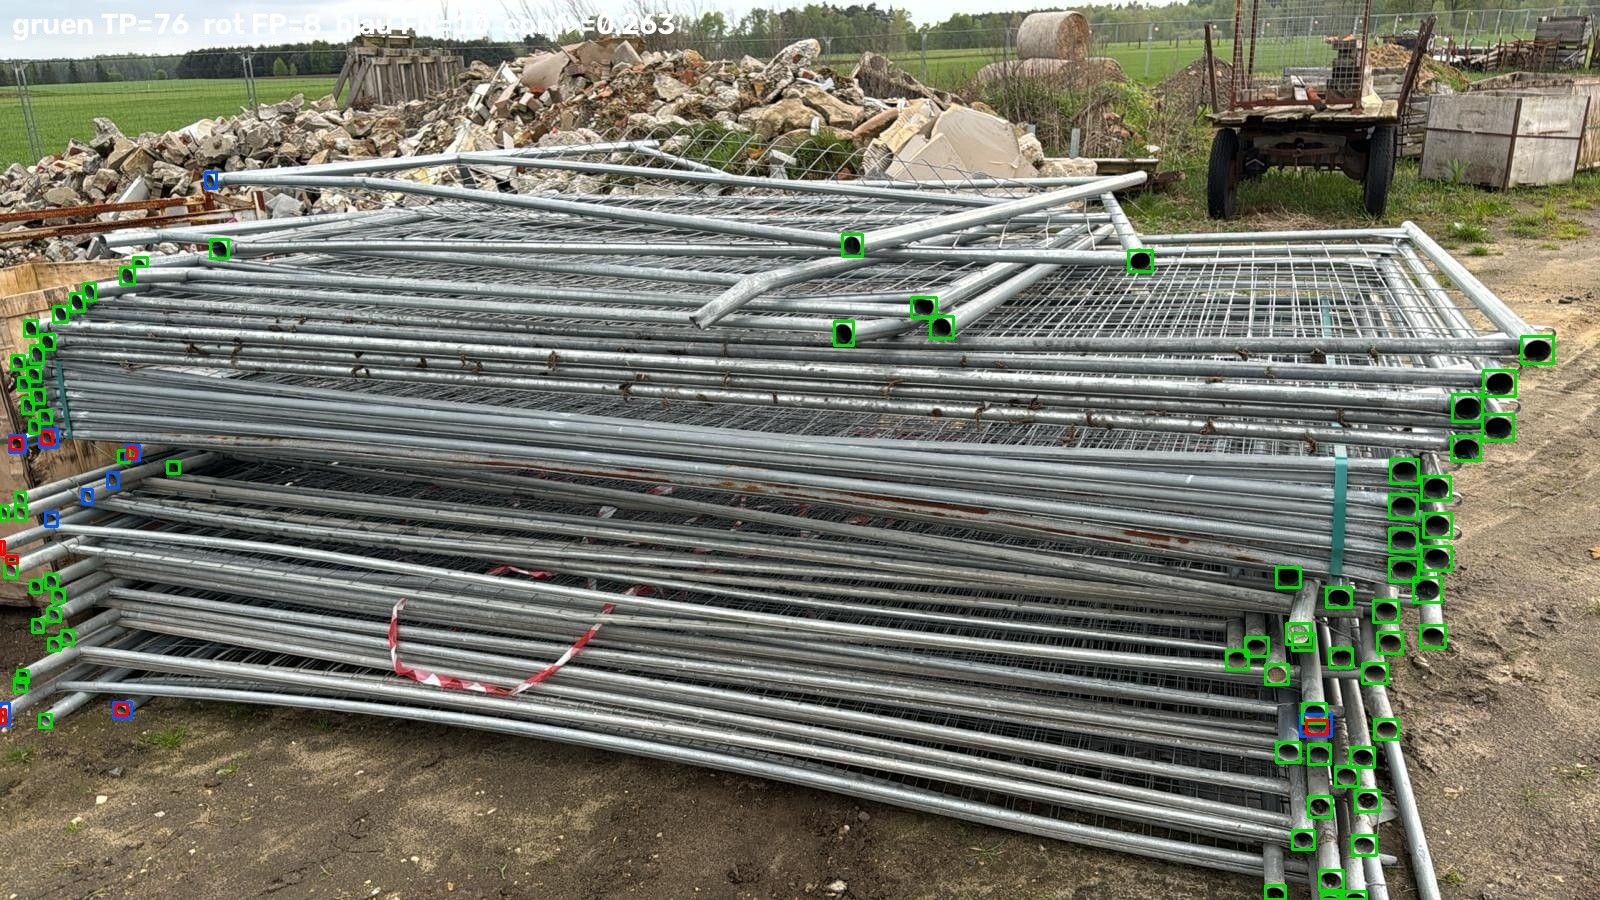
\includegraphics[width=\textwidth]{abbildungen/qual_test.jpg}
\caption[Qualitative Ergebnisse]{Qualitative Ergebnisse auf \code{val} (oben)
und \code{test} (unten). Grün = Treffer, rot = Falsch-Positiv, blau =
Falsch-Negativ. Im oberen Bild sitzen mehrere rot markierte Detektionen auf
erkennbaren Rohröffnungen, die in der Ground Truth fehlen; im unteren liegen rote
und blaue Boxen an mehreren Stellen nahezu deckungsgleich -- dasselbe Objekt zählt
dort doppelt als Fehler (Abschnitte~\ref{sec:fehleranalyse}
und~\ref{sec:boxversatz}).}
\label{abb:qualitativ}
\end{figure}

\section{Der Sim-to-Real-Abstand}
\label{sec:simtoreal}

Der Split \code{sval} besteht aus 400 synthetischen Bildern derselben Pipeline,
aber mit anderem Seed. Er ist damit die einzige Möglichkeit, die beiden
Fehlerquellen zu trennen: \emph{Kann das Modell die Aufgabe überhaupt?} und
\emph{überträgt es sich auf echte Bilder?}

\begin{equation}
\underbrace{0{,}982}_{\text{\code{sval}}}
\;-\;
\underbrace{0{,}886 \,/\, 0{,}888}_{\text{\code{val} / \code{test}}}
\;=\;
\textbf{9{,}6 bzw.\ 9{,}5 Prozentpunkte } \mAPfifty{}
\end{equation}

Bei \mAPall{} ist der Abstand mit 23,1 (\code{val}) bzw.\ 39,1 (\code{test})
Prozentpunkten deutlich größer -- was nach dem vorigen Abschnitt zu erwarten
ist, da die synthetischen Objekte im Median mit 22,5\px{} etwas größer sind als
die von \code{test}.

\absatz{Interpretation in beide Richtungen.} Der Abstand ist eine gute Nachricht
in zwei Hinsichten:

\begin{itemize}
  \item Er ist \textbf{klein genug}, dass das Verfahren praktisch funktioniert.
  Ein rein synthetisch trainiertes Modell verliert auf echten Bildern etwa
  10\PP{} -- und liegt damit noch in einem Bereich, in dem der Zählfehler unter
  3\,\% bleibt.
  \item Er ist \textbf{groß genug}, um zu belegen, dass das Netz \emph{nicht}
  bloß Einfügeartefakte gelernt hat. Wäre die Pipeline an einer der Signaturen
  S1--S6 durchlässig, so wäre \code{sval} nahezu perfekt ($>0{,}99$) und die
  realen Bilder katastrophal. Genau dieses Muster tritt nicht auf.
\end{itemize}

Dieses Argument ist der einzige \emph{direkte} empirische Hinweis darauf, dass
die Anti-Abkürzungs-Maßnahmen aus Abschnitt~\ref{sec:photometrie} und
\ref{sec:globalstufe} greifen. Es ist ein Indiz und kein Beweis: Ein
kontrollierter Nachweis müsste je Signatur einen eigenen Trainingslauf
vergleichen. Die Grenzen dieses Schlusses werden in
Abschnitt~\ref{sec:tragend} bilanziert.

\section{Experiment 1: die Inferenzauflösung}
\label{sec:imgsz}

Die Inferenzauflösung ist der einzige hier untersuchte Parameter, der nach dem
Training noch frei ist, und deshalb der einzige, dessen Wert gemessen statt
begründet wird. Gemustert werden neun Stufen zwischen 640 und 2464\px{} sowie
der native Maßstab. Ausgewählt wird die Stufe mit dem höchsten \mAPall{} auf
\code{val}, und zwar ausschließlich dort; der so gefundene Wert wird unverändert
auf beide Splits angewandt -- eine Wahl je Split wäre eine
Hyperparameterselektion auf dem Testsatz und würde dessen Zahlen wertlos machen.
Das Kriterium ist bewusst \mAPall{} und nicht \mAPfifty{}, weil es die
Lokalisierungsgüte mitbewertet; es stand vor den Läufen fest und gilt
unverändert für alle drei in Abschnitt~\ref{sec:modelle} verglichenen Modelle.
Für die Baseline fallen beide Metriken auseinander: \mAPfifty{} ist bei 1600 am
höchsten, \mAPall{} bei 1920; gewählt wurde daher 1920.

\begin{table}[htbp]
\centering
\caption[Sweep der Inferenzauflösung]{Sweep der Inferenzauflösung
\code{imgsz}. \enquote{pred} ist die Zahl der Detektionen am Betriebspunkt,
\enquote{gt} die Zahl der Ground-Truth-Objekte. Nativer Maßstab ist 2464
(\code{val}) bzw.\ 1600 (\code{test}).}
\label{tab:imgsz}
\footnotesize
\begin{tabular}{@{}lrrrrrrrr@{}}
\toprule
\textbf{Split} & \code{imgsz} & \mAPfifty{} & \mAPall{} & \textbf{bestes F1} &
$R$ & $P$ & \textbf{mittl.\ IoU} & \textbf{pred/gt} \\
\midrule
\code{val} & 640  & 0{,}435 & 0{,}201 & 0{,}507 & 0{,}398 & 0{,}700 & 0{,}711 & 50/88 \\
\code{val} & 800  & 0{,}793 & 0{,}428 & 0{,}768 & 0{,}659 & 0{,}921 & 0{,}737 & 63/88 \\
\code{val} & 960  & 0{,}852 & 0{,}498 & 0{,}840 & 0{,}773 & 0{,}919 & 0{,}773 & 74/88 \\
\code{val} & 1024 & 0{,}868 & 0{,}546 & 0{,}876 & 0{,}841 & 0{,}914 & 0{,}802 & 81/88 \\
\code{val} & 1280 & 0{,}887 & 0{,}577 & 0{,}861 & 0{,}841 & 0{,}881 & 0{,}808 & 84/88 \\
\code{val} & 1600 & \textbf{0{,}904} & 0{,}606 & 0{,}850 & 0{,}898 & 0{,}806 & 0{,}820 & 98/88 \\
\code{val} & 1920 & 0{,}893 & 0{,}613 & 0{,}851 & 0{,}909 & 0{,}800 & 0{,}830 & 100/88 \\
\code{val} & 2240 & 0{,}880 & 0{,}588 & 0{,}843 & 0{,}852 & 0{,}833 & 0{,}825 & 90/88 \\
\code{val} & 2464 & 0{,}886 & 0{,}597 & 0{,}862 & 0{,}852 & 0{,}872 & 0{,}824 & 86/88 \\
\midrule
\code{test} & 640  & 0{,}524 & 0{,}335 & 0{,}620 & 0{,}465 & 0{,}930 & 0{,}790 & 43/86 \\
\code{test} & 800  & 0{,}665 & 0{,}363 & 0{,}699 & 0{,}593 & 0{,}850 & 0{,}753 & 60/86 \\
\code{test} & 960  & 0{,}889 & 0{,}430 & 0{,}855 & 0{,}826 & 0{,}887 & 0{,}733 & 80/86 \\
\code{test} & 1024 & 0{,}882 & 0{,}459 & 0{,}841 & 0{,}767 & 0{,}930 & 0{,}740 & 71/86 \\
\code{test} & 1280 & 0{,}900 & 0{,}449 & 0{,}907 & 0{,}849 & 0{,}973 & 0{,}744 & 75/86 \\
\code{test} & 1600 & 0{,}888 & 0{,}437 & 0{,}894 & 0{,}884 & 0{,}905 & 0{,}748 & 84/86 \\
\code{test} & 1920 & \textbf{0{,}928} & 0{,}448 & 0{,}917 & 0{,}895 & 0{,}939 & 0{,}745 & 82/86 \\
\code{test} & 2240 & 0{,}928 & 0{,}457 & 0{,}920 & 0{,}872 & 0{,}974 & 0{,}744 & 77/86 \\
\code{test} & 2464 & 0{,}927 & 0{,}454 & 0{,}928 & 0{,}895 & 0{,}963 & 0{,}743 & 80/86 \\
\bottomrule
\end{tabular}
\end{table}

\begin{figure}[htbp]
\centering
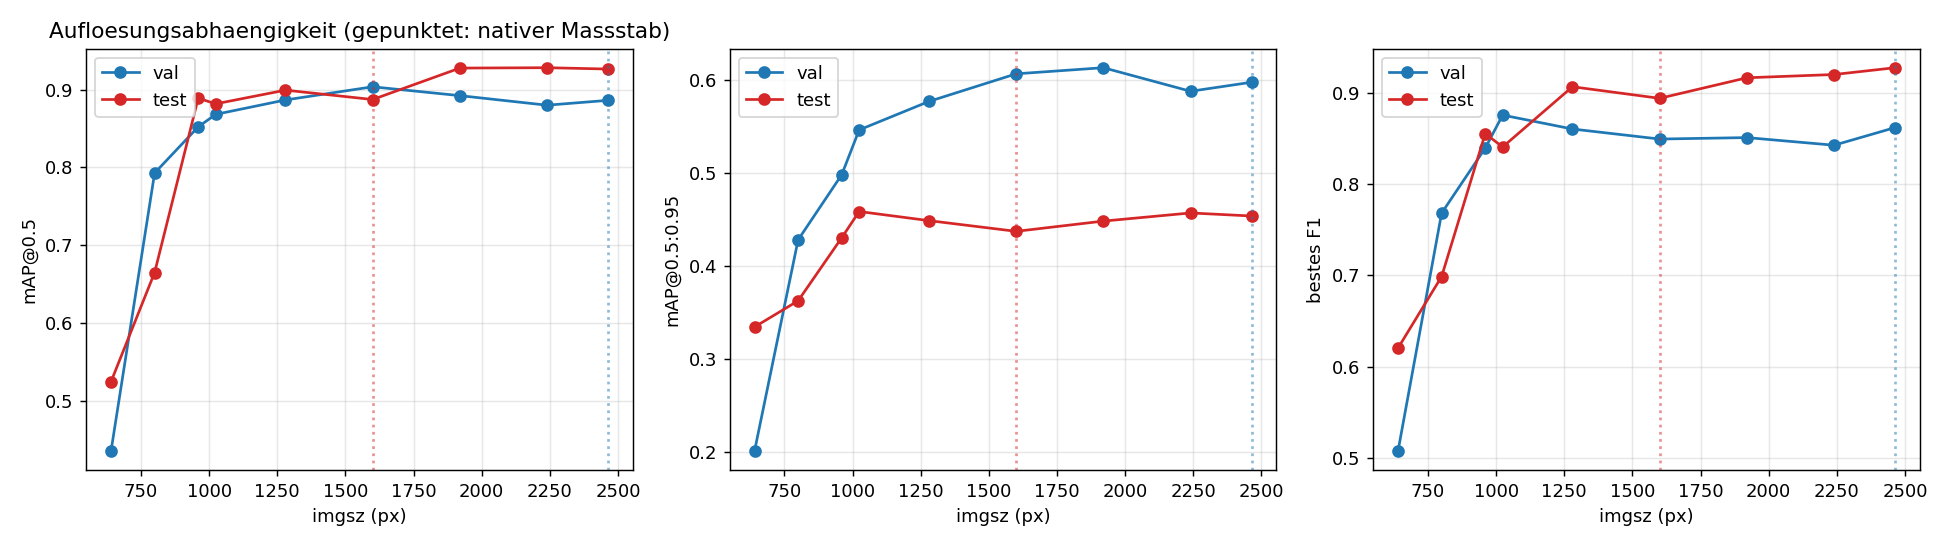
\includegraphics[width=\textwidth]{abbildungen/imgsz_sweep.png}
\caption[Sweep der Inferenzauflösung]{Sweep der Inferenzauflösung. Von 640 auf
1600\px{} verdoppelt sich \mAPfifty{} auf \code{val}; ab etwa 1280\px{} sättigt
die Kurve.}
\label{abb:imgsz}
\end{figure}

\absatz{Der größte Einzeleffekt der gesamten Arbeit.} Von \code{imgsz}~640 auf
1600 steigt \mAPfifty{} auf \code{val} von 0,435 auf 0,904 -- eine Verdopplung.
Dieser Effekt ist größer als jede einzelne Entscheidung in der
Augmentierungspipeline. Das ist ein für die Praxis unbequemes, aber wichtiges
Ergebnis: Die sorgfältigste Datensynthese wird wirkungslos, wenn die
Inferenzauflösung falsch gewählt ist.

Die Erklärung ist rein geometrisch und wurde in
Abschnitt~\ref{sec:effektivgroesse} vorhergesagt. Bei \code{imgsz}~640 wird das
2459\px{} breite \code{val}-Bild um den Faktor 0,26 verkleinert; die Objekte
schrumpfen von 20--36\px{} auf 5--9\px{} und liegen damit unter dem Stride~8 der
feinsten Detektionsebene. Der Rückruf bricht entsprechend auf 0,398 ein: Das
Modell \emph{findet} die Objekte nicht mehr, es lokalisiert sie nicht bloß
schlechter.

\absatz{Das Optimum liegt nicht am nativen Maßstab.} Für \code{test} (1600\px{}
breit) ist \code{imgsz}~1920--2464 -- also eine \emph{Hochskalierung} um Faktor
1,2--1,5 -- spürbar besser als der native Maßstab (0,928 gegen 0,888). Der Grund
liegt in der Trainingsverteilung: Der Generator erzeugt Objekte mit Median
22,5\px{}, \code{test} hat aber nur 19,6\px{} Median. Eine leichte
Hochskalierung schiebt die Testobjekte in die Mitte der Trainingsverteilung.
Daraus folgt eine unmittelbar anwendbare Regel:

\begin{quote}
\textbf{Praktische Empfehlung.} Nicht auf den nativen Maßstab skalieren, sondern
so, dass die erwartete Objektgröße im Netzeingang etwa dem Median der
Trainingsverteilung entspricht -- hier rund 22\px{}.
\end{quote}

Damit ist auch der Zusammenhang zur Pipeline benannt: Die Wahl des
Objektgrößenbereichs im Generator (Abschnitt~\ref{sec:instanzgeometrie}) und die
Wahl der Inferenzauflösung sind \emph{nicht} unabhängig. Wer den einen Parameter
verschiebt, muss den anderen mitverschieben.

\section{Die übrigen Inferenzparameter}
\label{sec:infparam}

Der Vollständigkeit halber wurden die weiteren Inferenzparameter bei
\code{imgsz}~1920 durchmustert. Das Ergebnis ist in allen Fällen unkritisch --
was selbst eine Aussage ist, weil es die Interpretation von
Abschnitt~\ref{sec:imgsz} stützt.

\begin{table}[htbp]
\centering
\caption[Übrige Inferenzparameter]{Übrige Inferenzparameter bei
\code{imgsz}~1920. TTA = Test-Time-Augmentation (Mehrfachskalen und
Spiegelung), FP16 = Inferenz in halber Genauigkeit.}
\label{tab:infparam}
\footnotesize
\resizebox{\textwidth}{!}{%
\begin{tabular}{@{}llrrrr@{}}
\toprule
\textbf{Parameter} & \textbf{Wert} & \code{val} \mAPfifty{} &
\code{val} \mAPall{} & \code{test} \mAPfifty{} & \code{test} \mAPall{} \\
\midrule
NMS-IoU & 0{,}30 & 0{,}897 & 0{,}620 & 0{,}933 & 0{,}453 \\
NMS-IoU & 0{,}45 & 0{,}895 & 0{,}616 & 0{,}931 & 0{,}450 \\
NMS-IoU & 0{,}70 (Std.) & 0{,}893 & 0{,}613 & 0{,}928 & 0{,}448 \\
NMS-IoU & 0{,}90 & 0{,}867 & 0{,}600 & 0{,}928 & 0{,}450 \\
\midrule
\code{max\_det} & 50   & 0{,}735 & 0{,}555 & 0{,}788 & 0{,}440 \\
\code{max\_det} & 100  & 0{,}885 & 0{,}637 & 0{,}944 & 0{,}493 \\
\code{max\_det} & 300 (Std.) & 0{,}892 & 0{,}617 & 0{,}930 & 0{,}457 \\
\code{max\_det} & 1000 & 0{,}893 & 0{,}613 & 0{,}928 & 0{,}448 \\
\midrule
TTA & aus  & 0{,}893 & 0{,}613 & 0{,}928 & 0{,}448 \\
TTA & \textbf{ein} & \textbf{0{,}914} & 0{,}618 & \textbf{0{,}934} & 0{,}472 \\
FP16 & ein & 0{,}893 & 0{,}613 & 0{,}928 & 0{,}448 \\
\bottomrule
\end{tabular}}
\end{table}

\begin{itemize}
  \item \textbf{NMS-IoU} (0,3--0,9): Spanne nur 3\PP{} \mAPfifty{}. Das war
  vorhersagbar: Benachbarte Rohrenden haben nach
  Tabelle~\ref{tab:anordnung} mindestens etwa 0,85 Durchmesser Abstand, ihre
  Boxen überlappen also kaum -- die NMS ist hier fast wirkungslos. Das ist
  gleichzeitig der Grund, warum die NMS-freie Inferenz von YOLO26
  (Abschnitt~\ref{sec:yolo26}) in \emph{diesem} Anwendungsfall weniger bringt,
  als die Argumentation in Abschnitt~\ref{sec:anwendung} erwarten lässt.
  \item \textbf{\code{max\_det}}: 50 ist katastrophal (\mAPfifty{} 0,735 statt
  0,893, Zählung 50/88), ab 100 gesättigt. Der Standardwert 300 reicht für diese
  Bilder, wäre bei einem großen Stapel aber eine stille Obergrenze -- deshalb
  wird für alle Messungen 1000 verwendet, damit die Metrik nie durch eine
  Kappungsgrenze verfälscht wird.
  \item \textbf{FP16}: bitidentische Ergebnisse zu FP32 bei etwa gleicher
  Laufzeit. Kein Grund, darauf zu verzichten, aber auch kein Gewinn.
  \item \textbf{TTA}: $+2{,}1$\PP{} \mAPfifty{} auf \code{val} und
  $+0{,}6$\PP{} auf \code{test}, bei deutlich besserer Zählung (100/88 $\to$
  90/88). Kostet etwa den doppelten Rechenaufwand. Für eine Zählanwendung, die
  nicht in Echtzeit laufen muss, lohnt sich das. Bemerkenswert ist, dass TTA
  hier im Kern Skalen- und Spiegelungsaugmentierung zur \emph{Inferenzzeit} ist
  \parencite{shanmugam2021} -- also dieselben Transformationen, die auch im
  Training verwendet werden.
\end{itemize}

\section{Experiment 2: Wie viel Verdeckung in den Trainingsdaten?}
\label{sec:ablation}

Dies ist das zentrale Augmentierungsexperiment der Arbeit. Die
Okklusionserzeugung ist die aufwendigste Einzelstufe der Pipeline -- sie
erfordert die Okkluder-Bibliothek, das Tiefenmodell und die exakte
Sichtbarkeitsrechnung. Die Frage ist, ob sich dieser Aufwand messbar auszahlt.

\subsection{Versuchsaufbau}

Drei Datensätze werden erzeugt, die sich \emph{ausschließlich} im
Verdeckungsgrad unterscheiden. Alles andere ist identisch: derselbe Seed,
dieselbe Bildzahl (3000), dieselben Objektpositionen, dieselben Hyperparameter,
30 Epochen.

\begin{table}[htbp]
\centering
\caption[Ablationsarme]{Die drei Ablationsarme. Der Rohrschaft hinter der
Stirnfläche bleibt in \emph{allen} Armen erhalten -- er ist physikalische
Randbedingung und keine Augmentierung. Variiert wird nur, wie stark verdeckt
wird.}
\label{tab:ablarme}
\footnotesize
\begin{tabularx}{\textwidth}{@{}L{0.15\textwidth}L{0.30\textwidth}X@{}}
\toprule
\textbf{Arm} & \textbf{Änderung gegenüber der Baseline} & \textbf{Bedeutung} \\
\midrule
\textbf{A0} keine Okklusion &
\code{img\_has\_bars} $= 0$, \code{img\_clutter} $= 0$,
\code{stub\_behind\_front} $= 1$ &
keine quer liegenden Stangen, keine Fremdkörper, kein Schaft kreuzt vor einer
Stirnfläche \\
\textbf{A1} Baseline &
Sollwerte aus Kapitel~\ref{kap:pipeline} &
0{,}65 / 0{,}35 / 0{,}75 \\
\textbf{A2} starke Okklusion &
\code{img\_has\_bars} $= 1$, \code{img\_clutter} $= 0{,}70$,
\code{stub\_behind\_front} $= 0{,}40$ &
in jedem Bild Stangen, mehr Fremdkörper, mehr quer vor dem Stapel liegende
Rohre \\
\bottomrule
\end{tabularx}
\end{table}

Die Kontrolle ist besser als bei einer gewöhnlichen Datensatz-Ablation: Weil der
Seed identisch ist, rendern alle drei Arme \textbf{genau dieselben 86\,617
Instanzen an denselben Positionen}. Der einzige Unterschied besteht darin,
wie viel davon verdeckt wird und -- als Folge -- wie viele Labels die
Sichtbarkeitsregel aus Abschnitt~\ref{sec:sichtbarkeit} verwirft.

\begin{table}[htbp]
\centering
\caption[Erzeugte Ablationsdatensätze]{Die drei erzeugten Datensätze (je 3000
Bilder, 86\,617 gerenderte Instanzen).}
\label{tab:abldaten}
\footnotesize
\resizebox{\textwidth}{!}{%
\begin{tabular}{@{}lrrrrr@{}}
\toprule
\textbf{Arm} & \textbf{Labels} & \textbf{mittl.\ Sichtbarkeit} &
\textbf{teilverdeckt} & \textbf{verworfen (Verdeckung)} &
\textbf{Bilder mit Stangen} \\
\midrule
A0 & 82\,950 & 0{,}977 & 12{,}0\,\% & 241 & 0\,\% \\
A1 & 68\,281 & 0{,}902 & 29{,}9\,\% & 15\,312 & 57{,}6\,\% \\
A2 & 55\,833 & 0{,}852 & 40{,}7\,\% & 28\,108 & 89{,}9\,\% \\
\bottomrule
\end{tabular}}
\end{table}

\begin{figure}[htbp]
\centering
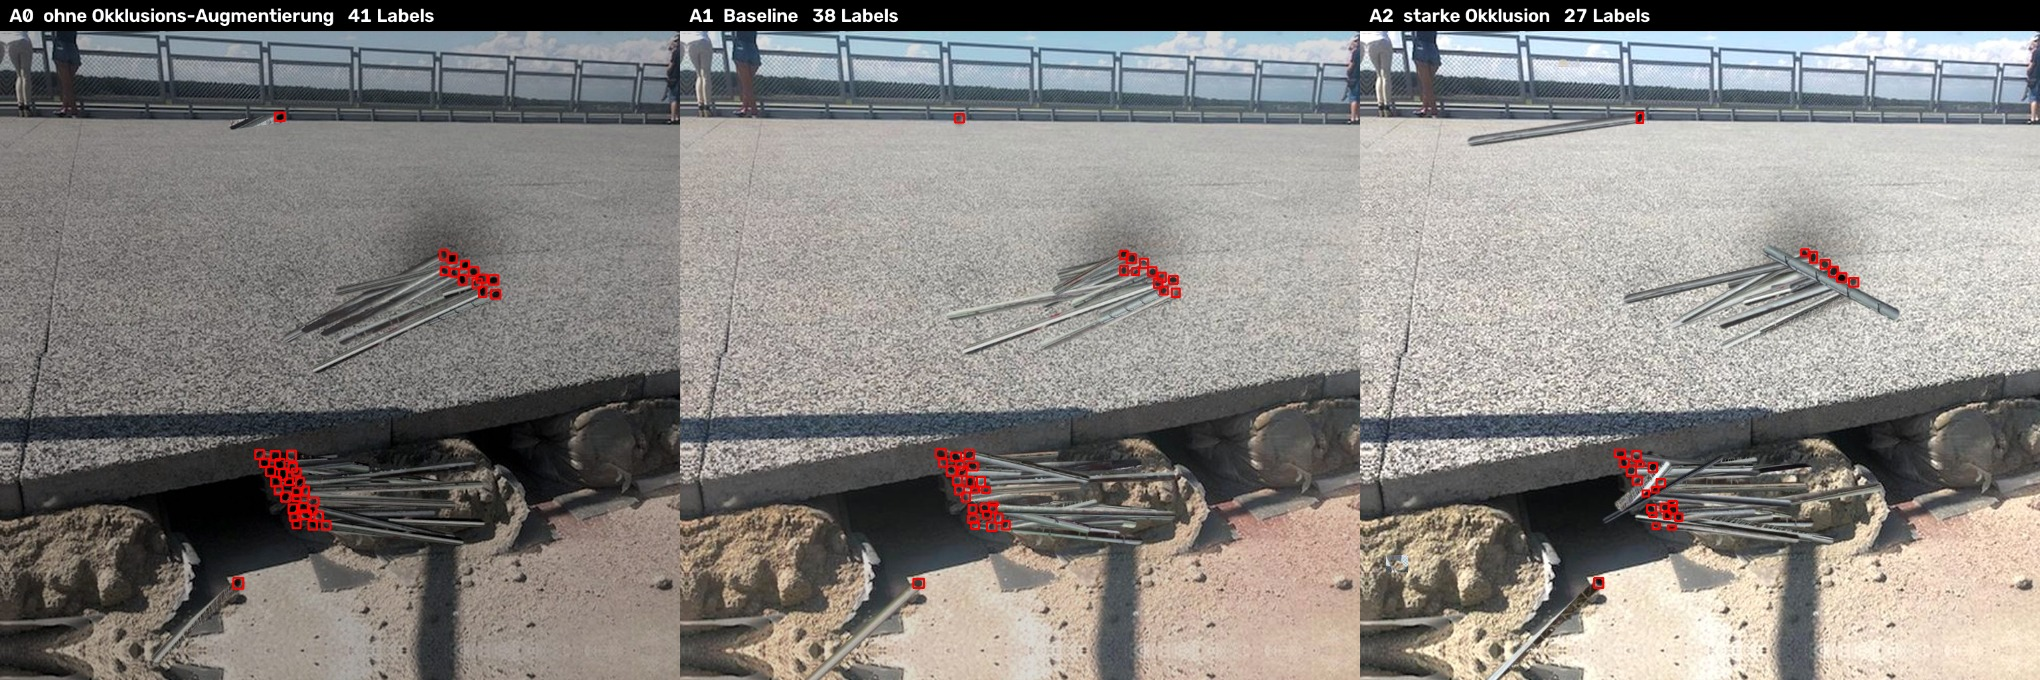
\includegraphics[width=\textwidth]{abbildungen/ablation_beispiele.jpg}
\caption[Die drei Ablationsarme]{Dasselbe Bild (identischer Seed) aus allen drei
Armen: A0 ohne Okklusion (links), A1 Baseline (Mitte), A2 starke Okklusion
(rechts). Die Objektpositionen sind identisch; es unterscheidet sich nur, wie
viel davon verdeckt ist -- und damit, wie viele Labels übrig bleiben.}
\label{abb:ablbeispiele}
\end{figure}

\subsection{Ergebnis}

\begin{table}[htbp]
\centering
\caption[Ergebnis der Okklusionsablation]{Ergebnis der Okklusionsablation,
nativer Maßstab. Alle sechs Metrikspalten sind über die drei Arme
\textbf{monoton}.}
\label{tab:ablergebnis}
\footnotesize
\resizebox{\textwidth}{!}{%
\begin{tabular}{@{}lrrrrrrr@{}}
\toprule
\textbf{Arm} & \textbf{Labels} &
\code{val} \mAPfifty{} & \code{val} \mAPall{} &
\code{test} \mAPfifty{} & \code{test} \mAPall{} & \code{test} F1 &
\code{test} Zählung \\
\midrule
A0 ohne     & 82\,950 & 0{,}888 & 0{,}606 & 0{,}899 & 0{,}418 & 0{,}896 & 77/86 \\
A1 Baseline & 68\,281 & 0{,}924 & 0{,}609 & 0{,}911 & 0{,}452 & 0{,}904 & 80/86 \\
A2 stark    & 55\,833 & \textbf{0{,}930} & \textbf{0{,}620} &
\textbf{0{,}919} & \textbf{0{,}454} & \textbf{0{,}910} & \textbf{81/86} \\
\bottomrule
\end{tabular}}
\end{table}

\begin{figure}[htbp]
\centering
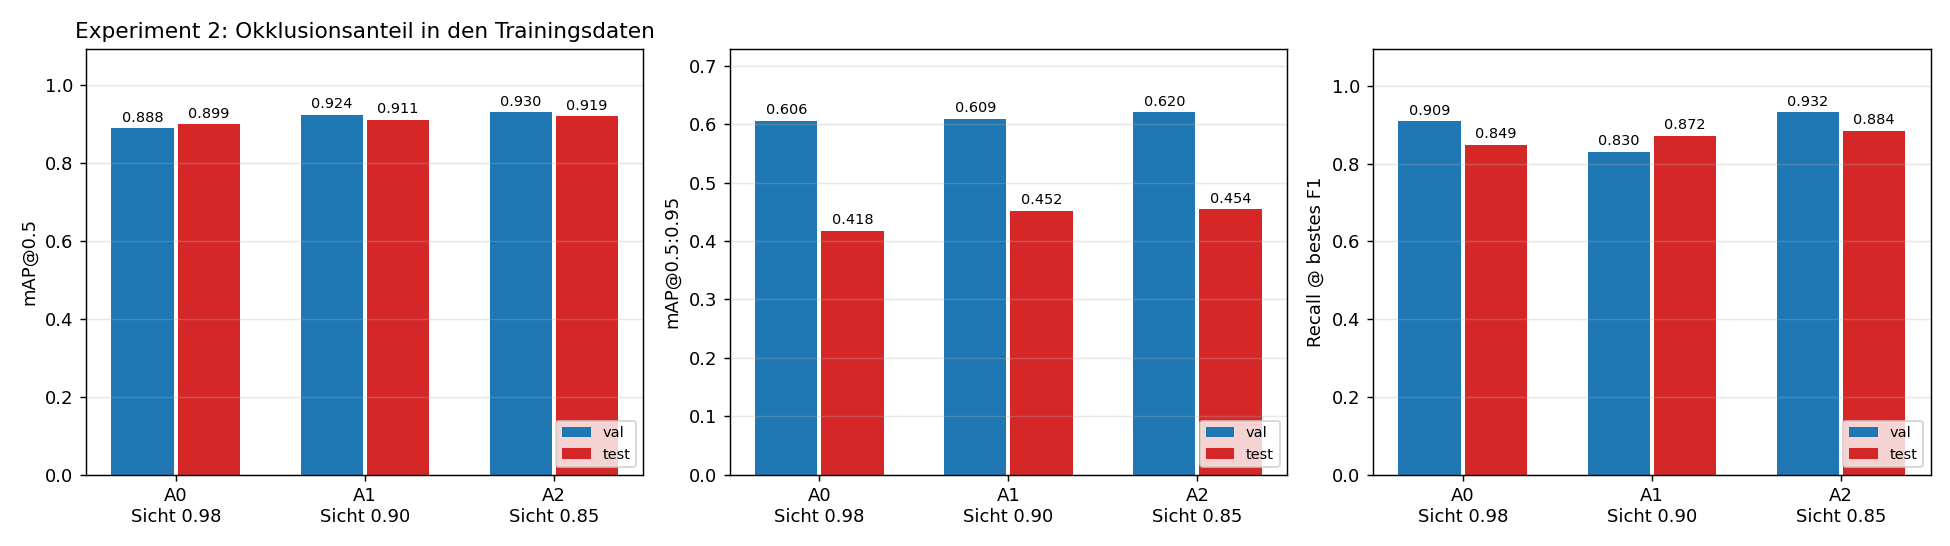
\includegraphics[width=\textwidth]{abbildungen/ablation.png}
\caption[Okklusionsablation]{Ergebnis der Okklusionsablation über die drei Arme.
Der Anstieg ist auf beiden Splits und in allen berichteten Metriken monoton.}
\label{abb:ablation}
\end{figure}

\absatz{Befund 1 -- der Effekt ist monoton.} Von A0 zu A2 steigen \mAPfifty{} um
2,0\PP{} und \mAPall{} um 3,6\PP{} auf dem unberührten Testbild. Der Anstieg
tritt in allen sechs Metrikspalten von Tabelle~\ref{tab:ablergebnis} und über
alle drei Stufen in derselben Richtung auf.

\absatz{Befund 2 -- der Gewinn entsteht \emph{gegen} einen Verlust an
Supervision.} A2 hat durch die stärkere Verdeckung \textbf{32,7\,\% weniger
Labels} als A0 (55\,833 gegen 82\,950 bei identischer Bildzahl und identischen
gerenderten Instanzen). Der Okklusionsvorteil überkompensiert also einen
deutlichen Verlust an Trainingssignal. Das ist der stärkste Einzelbeleg dafür,
dass die Okklusionsstufe kein Beiwerk ist: Wären die zusätzlichen Labels
wertvoller als die zusätzliche Schwierigkeit, müsste A0 gewinnen.

\absatz{Befund 3 -- ohne Verdeckung ist die Aufgabe zu leicht.} Ein zweiter
Befund steckt im Trainingsverlauf: \textbf{A0 erreichte sein bestes Modell
bereits in Epoche~3} und verbesserte sich in den folgenden 20 Epochen nicht mehr
(Early Stopping bei Epoche~23). A1 und A2 verbesserten sich bis zur letzten
Epoche~30 durchgehend. Ohne Verdeckung sättigt das Modell sofort und passt sich
danach nur noch an die synthetische Verteilung an -- dieselbe Schere wie in
Abschnitt~\ref{sec:trainingsverlauf}, nur früher einsetzend.

\absatz{Einordnung in die Literatur.} Der Befund ist mit den Ergebnissen zu
Cutout und Random Erasing verträglich \parencite{devries2017cutout,zhong2020erasing},
geht aber über sie hinaus: Dort wird Bildinhalt gelöscht und das Label
beibehalten, hier verdeckt ein Objekt mit eigener Textur, und das Label wird bei
zu starker Verdeckung entfernt. Die entstehenden Beispiele sind damit sowohl
schwierigere Positive als auch korrekte harte Negative -- letzteres ist bei
generischem Cutout nicht erreichbar. Das Ergebnis stützt zudem die Beobachtung
von \textcite{wang2017afastrcnn}, dass Okklusion für Detektoren ein wirksames
Trainingssignal ist.

\subsection{Einschränkungen dieses Experiments}
\label{sec:ableinschraenkung}

Die Einschränkungen sind erheblich und werden hier ausdrücklich genannt:

\begin{enumerate}
  \item \textbf{Der Effekt liegt innerhalb des Konfidenzintervalls.} Das
  Bootstrap-Intervall für \mAPfifty{} beträgt $\pm 0{,}05$ (\code{val}) bzw.\
  $\pm 0{,}04$ (\code{test}) und ist damit breiter als der gemessene Unterschied
  von 0,02--0,04 (Abschnitt~\ref{sec:bootstrap}). Belastbar ist nicht die
  einzelne Differenz, sondern die \emph{Konsistenz}: dieselbe Richtung in drei
  Metriken $\times$ zwei Splits $\times$ drei Stufen. Bei reinem Rauschen wäre
  eine solche durchgehende Monotonie unwahrscheinlich; ein formaler
  Signifikanznachweis ist mit je einem Bild pro Split aber nicht möglich.
  \item \textbf{Labelzahl und Okklusionsanteil sind nicht entkoppelt.} Mehr
  Verdeckung heißt zwangsläufig mehr verworfene Labels. Der Vergleich mischt
  also zwei Effekte, die sich hier zufällig gegenläufig verhalten. Ein saubereres
  Nachfolgeexperiment müsste die Bildzahl je Arm so anpassen, dass alle Arme
  gleich viele Labels enthalten.
  \item \textbf{A1 und A2 waren nach 30 Epochen nicht auskonvergiert.} Ihr
  Vorsprung könnte bei längerem Training größer werden -- die Aussage ist also
  konservativ, aber nicht abgeschlossen.
  \item \textbf{Eine Metrik ist nicht monoton.} \mAPseven{} auf \code{val}
  verläuft 0,812 / 0,760 / 0,775 und fällt damit aus dem Muster. Der Wert ist bei
  27\px{} großen Objekten besonders empfindlich gegenüber wenigen
  Boxabweichungen (Gleichung~\eqref{eq:ioushift}); die Aussage der Ablation
  betrifft das Finden der Objekte, nicht die Präzision der Boxen.
  \item \textbf{Ein Nebenbefund.} A1 und A2 (3000 Bilder, 30 Epochen) schlagen
  den Hauptlauf (6000 Bilder, bestes Modell aus Epoche~10) auf beiden Splits.
  Auch das liegt im Rauschen, deutet aber darauf hin, dass zusätzliche
  synthetische Bilder ab einer gewissen Menge nichts mehr bringen: Die Vielfalt
  ist durch die neun Ausschnitte begrenzt, nicht durch die Bildzahl.
\end{enumerate}

\section{Experiment 3: Modellfamilie}
\label{sec:modelle}

Dieses Experiment prüft nach, was Kapitel~\ref{kap:theorie} theoretisch
begründet: dass YOLO26 -- und insbesondere die Variante mit zusätzlichem
P2-Detektionskopf -- für kleine, dicht gepackte Objekte besser geeignet sein
sollte. Alle drei Läufe verwenden identisches Budget, identische
Hyperparameter und denselben Datensatz.

\begin{table}[htbp]
\centering
\caption[Modellfamilienvergleich]{Modellfamilienvergleich. Oben nativer
Maßstab, unten bei der je Modell auf \code{val} gewählten Auflösung
(\code{yolo11s}: 1920, \code{yolo26s}: 1600, \code{yolo26s-p2}: 1920). Die Wahl
erfolgte nach \mAPall{} und ausschließlich auf \code{val}; \code{test} blieb
unberührt.}
\label{tab:modelle}
\footnotesize
\resizebox{\textwidth}{!}{%
\begin{tabular}{@{}lrrrrrrr@{}}
\toprule
\textbf{Modell} & \textbf{Par.\ (M)} &
\code{val} \mAPfifty{} & \code{test} \mAPfifty{} & \code{test} \mAPseven{} &
\code{test} \mAPall{} & \code{test} F1 & \code{test} Zählung \\
\midrule
\multicolumn{8}{@{}l}{\itshape nativer Maßstab}\\
\code{yolo11s}    & 9{,}43 & 0{,}886 & 0{,}888 & 0{,}320 & 0{,}437 & 0{,}894 & 84/86 \\
\code{yolo26s}    & 9{,}95 & 0{,}931 & 0{,}905 & 0{,}333 & 0{,}427 & 0{,}888 & 83/86 \\
\code{yolo26s-p2} & 9{,}66 & 0{,}936 & \textbf{0{,}941} & \textbf{0{,}387} &
0{,}450 & \textbf{0{,}933} & 79/86 \\
\midrule
\multicolumn{8}{@{}l}{\itshape bei der auf \code{val} gewählten \code{imgsz}}\\
\code{yolo11s} (1920)    & 9{,}43 & 0{,}893 & 0{,}928 & -- & 0{,}448 & 0{,}917 & 82/86 \\
\code{yolo26s} (1600)    & 9{,}95 & 0{,}939 & 0{,}905 & -- & 0{,}427 & 0{,}888 & 83/86 \\
\code{yolo26s-p2} (1920) & 9{,}66 & \textbf{0{,}940} & \textbf{0{,}947} & -- &
0{,}449 & \textbf{0{,}934} & 81/86 \\
\bottomrule
\end{tabular}}
\end{table}

\absatz{Interpretation.} Die theoretische Erwartung bestätigt sich: Bei
praktisch identischer Parameterzahl erreicht \code{yolo26s-p2} auf dem
unberührten Testbild \mAPfifty{} = 0,941 statt 0,888. Der Gewinn entsteht dabei
\emph{nicht} über die Boxpräzision: Die mittlere Treffer-IoU sinkt sogar leicht
(0,748 auf 0,728). Er entsteht über die Trennung von Objekt und Hintergrund --
die Precision am Betriebspunkt steigt von 0,905 auf 0,975 bei ebenfalls leicht
höherem Rückruf (0,884 auf 0,895). Das ist mit der Argumentation aus
Abschnitt~\ref{sec:ioukleinobjekt} konsistent: Ein zusätzlicher P2-Kopf mit
Stride~4 senkt die Auflösungsgrenze, an der ein Objekt überhaupt detektierbar
ist; er macht aber die Boxregression bei 20\px{}-Objekten nicht genauer. Der
Preis ist der Speicherbedarf: Die P2-Variante belegte im Training rund die
2,6-fache GPU-Speichermenge.

\absatz{Ein Vorbehalt für die Zählanwendung.} Der Vorteil in \mAPfifty{} setzt
sich nicht in einen besseren Zählfehler um: Am F1-optimalen Betriebspunkt zählt
\code{yolo26s-p2} auf \code{test} 79 statt 86 Objekte (Fehler 8,1\,\%),
\code{yolo11s} dagegen 84 (2,3\,\%). Die Ursache ist die Schwellenwahl: Das
F1-Optimum von \code{yolo26s-p2} liegt bei $c^* = 0{,}379$ gegenüber
$0{,}263$, tauscht also Rückruf gegen Precision. Da F1 beide Fehlerarten
gleich gewichtet, der Zählfehler sich aber aus ihrer \emph{Differenz} ergibt,
sind die beiden Optima nicht identisch. Für eine Zählanwendung ist der
Betriebspunkt daher direkt auf den Zählfehler zu optimieren und nicht auf F1 --
eine Einsicht, die für alle Modelle gilt und in dieser Arbeit bewusst nicht
umgesetzt wurde, weil eine auf \code{val} kalibrierte Zählschwelle die
Aussagekraft der \code{test}-Zahlen geschwächt hätte.

\absatz{Konsequenz und ehrliche Einordnung.} Die Wahl der Modellfamilie war
damit die schwächste Einzelentscheidung der Arbeit -- sie war zunächst
konservativ und unbelegt getroffen. \code{yolo11s} bleibt als dokumentierte
Baseline stehen, weil auf ihr die Experimente~1 und 2 gerechnet wurden; für einen
produktiven Einsatz wäre \code{yolo26s-p2} zu wählen. Für die
Augmentierungsergebnisse dieser Arbeit ändert das nichts: Alle drei Modelle haben
dieselben Strides auf P3/P4/P5, und die Ablation vergleicht Datensätze bei
identischem Modell.

\section{Statistische Belastbarkeit}
\label{sec:bootstrap}

Nach Befund~10 liegt je Split nur \emph{ein} Bild vor. Eine mAP-Angabe auf 88
Objekten ist eine Punktschätzung mit erheblicher Streuung, und ein gewöhnlicher
Bootstrap über Bilder ist nicht möglich. Verwendet wird daher ein
\textbf{räumlicher Block-Bootstrap}: Das Bild wird in Kacheln zerlegt, und es
wird über Kacheln mit Zurücklegen neu gezogen (400 Wiederholungen). Das Verfahren
entspricht dem Block-Bootstrap für abhängige Beobachtungen
\parencite{kuensch1989,efron1993}; die Blockbildung ist nötig, weil benachbarte
Objekte nicht unabhängig sind -- sie teilen Beleuchtung, Schärfe und
Verdeckungssituation.

\begin{table}[htbp]
\centering
\caption[Bootstrap-Konfidenzintervalle]{Bootstrap-Konfidenzintervalle für
\mAPfifty{}, 400 Wiederholungen über räumliche Kacheln.}
\label{tab:bootstrap}
\small
\begin{tabular}{@{}lrrrr@{}}
\toprule
\textbf{Split} & \textbf{Mittel} & \textbf{Std} & \textbf{95\,\%-KI} &
\textbf{Kacheln} \\
\midrule
\code{val}  & 0{,}892 & 0{,}051 & $[0{,}766;\ 0{,}965]$ & 23 \\
\code{test} & 0{,}911 & 0{,}036 & $[0{,}844;\ 0{,}974]$ & 25 \\
\bottomrule
\end{tabular}
\end{table}

Die Intervalle sind breit -- rund $\pm 0{,}05$ bzw.\ $\pm 0{,}04$. Alle in
diesem Kapitel berichteten Unterschiede unterhalb dieser Größenordnung sind
daher als Hinweis und nicht als Nachweis zu lesen. Das betrifft die
Okklusionsablation (Abschnitt~\ref{sec:ableinschraenkung}) und den
Modellvergleich; es betrifft \emph{nicht} den Auflösungseffekt aus
Abschnitt~\ref{sec:imgsz}, dessen Größe von 47\PP{} das
Intervall um ein Vielfaches übersteigt.

\section{Fehleranalyse}
\label{sec:fehleranalyse}

Aus den Qualitativbildern (Abbildung~\ref{abb:qualitativ}) lassen sich die
Fehler nach Ursache ordnen.

\absatz{Falsch-Negative} treten fast ausschließlich auf bei
\begin{itemize}
  \item sehr kleinen Objekten am linken Bildrand von \code{test}
  (12--15\px{}) -- also am unteren Rand der in
  Gleichung~\eqref{eq:effskala} abgedeckten Größenspanne,
  \item stark verdeckten Enden tief im Stapel -- also genau dort, wo die
  Pipeline nach Abschnitt~\ref{sec:sichtbarkeit} auch kein Label mehr vergäbe,
  \item Enden ohne sichtbaren hellen Kranz, die vollständig im Schatten liegen.
  Dies ist der Fehlertyp, der auf die verbleibende Domänenlücke zurückgeht: Alle
  vier Clean Plates sind bei diffusem Licht aufgenommen
  (Abschnitt~\ref{sec:hintergruende}).
\end{itemize}

\absatz{Falsch-Positive} haben auf den beiden Bildern \emph{unterschiedliche}
Ursachen, und die Unterscheidung ist nicht kosmetisch. Auf \code{val} haben 9 der
11 Falsch-Positiven keinerlei Überlappung mit einer Ground-Truth-Box; ein Teil
von ihnen sitzt auf erkennbaren Rohröffnungen, die in der Annotation fehlen. Bei
88 handannotierten Objekten schlägt jede fehlende Annotation mit etwa 1,1\PP{}
Precision zu Buche -- die berichteten Precision-Werte sind daher eher eine
\textbf{Untergrenze} als eine Punktschätzung. Die übrigen entstehen an dunklen
Löchern im Maschendraht und an Schattenspalten zwischen Rohren, genau die
Strukturen, gegen die die Negativbilder aus Abschnitt~\ref{sec:negative}
gerichtet sind; dass sie dort noch auftreten, spricht dafür, dass deren Anteil
von 9,7\,\% eher an der Untergrenze des Sinnvollen liegt.

Auf \code{test} liegt der Fall völlig anders: Dort sind \textbf{sechs der acht
Falsch-Positiven} Detektionen, die auf einem annotierten Objekt sitzen und die
Zuordnungsschwelle nur knapp verfehlen (IoU 0,401 bis 0,497, in zwei Fällen um
weniger als 0,005). Sie erscheinen im Qualitativbild als rote Box direkt neben
oder in einer blauen -- dasselbe Objekt wird gleichzeitig als Falsch-Positiv und
als Falsch-Negativ gezählt. Der nächste Abschnitt geht dem nach.

\section{Ein systematischer Größenversatz der Boxen}
\label{sec:boxversatz}

Eine Detektion gilt nur als Treffer, wenn ihre IoU mit der Ground-Truth-Box
mindestens 0,5 beträgt; liegt sie darunter, bleibt die Detektion unzugeordnet und
die Ground-Truth-Box unbedient. Auf \code{test} ergeben sich dadurch aus sechs
gefundenen Objekten zwölf Fehler. Senkt man allein die Zuordnungsschwelle von
0,50 auf 0,40, so ergeben sich 81 Treffer, 2 Falsch-Positive und 5
Falsch-Negative statt 75/8/11.

\begin{table}[htbp]
\centering
\caption[Größenversatz der Boxen]{Oben: Vergleich der vorhergesagten mit der
annotierten Boxgröße für alle Detektionen, die eindeutig auf einem annotierten
Objekt sitzen ($\mathrm{IoU} > 0{,}3$); als Boxgröße dient
$\sqrt{\text{Fläche}}$. Unten: Sensitivitätsrechnung mit um den medianen
Fehlbetrag je Seite aufgeweiteten Boxen -- \emph{kein} Ergebnis eines neuen
Trainings, sondern eine Obergrenzenschätzung.}
\label{tab:boxversatz}
\footnotesize
\begin{tabular}{@{}llrrrrr@{}}
\toprule
\multicolumn{7}{@{}l}{\itshape gemessener Versatz}\\
\textbf{Split} & & \textbf{Paare} & \textbf{Objekt-\Oe} &
\textbf{pred/GT} & \textbf{GT $-$ pred} & \textbf{Zentrumsversatz} \\
\midrule
\code{test} (real)        & &   82 & 22,3\px & 0,884 & $+2{,}53$\px & 0,049\,\Oe \\
\code{val} (real)         & &   75 & 27,5\px & 0,961 & $+1{,}16$\px & 0,054\,\Oe \\
\code{sval} (synthetisch) & & 1064 & 22,0\px & \textbf{1,012} & $-0{,}29$\px & -- \\
\midrule
\multicolumn{7}{@{}l}{\itshape Sensitivitätsrechnung}\\
 & & \mAPfifty{} & \mAPseven{} & \mAPall{} & \textbf{bestes F1} &
\textbf{mittl.\ IoU} \\
\midrule
\code{test} & unverändert       & 0,887 & 0,320 & 0,437 & 0,894 & 0,748 \\
\code{test} & Boxen aufgeweitet & \textbf{0,951} & \textbf{0,714} &
\textbf{0,604} & \textbf{0,959} & \textbf{0,805} \\
\code{val}  & unverändert       & 0,886 & 0,793 & 0,597 & 0,862 & 0,824 \\
\code{val}  & Boxen aufgeweitet & 0,886 & 0,812 & 0,622 & 0,862 & 0,835 \\
\bottomrule
\end{tabular}
\end{table}

\begin{figure}[htbp]
\centering
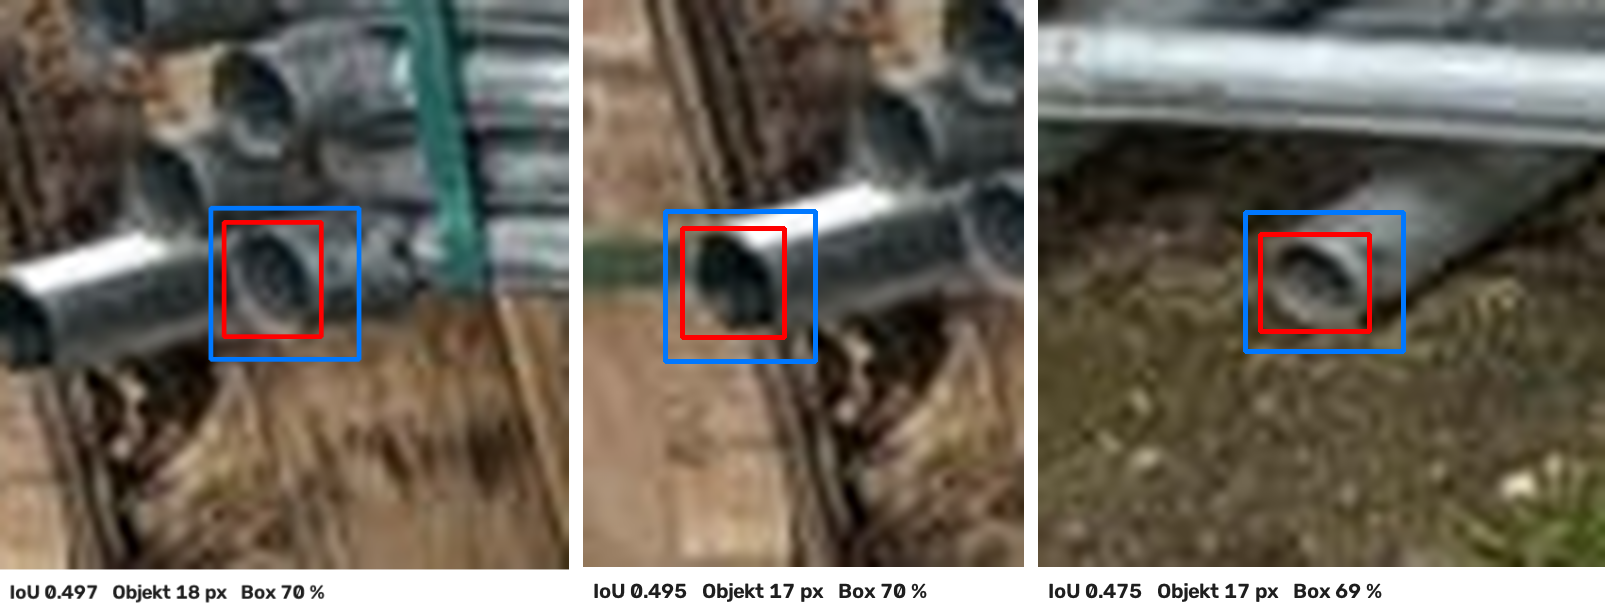
\includegraphics[width=\textwidth]{abbildungen/boxversatz.png}
\caption[Rote und blaue Box am selben Objekt]{Drei der sechs betroffenen Stellen
aus dem Testbild, neunfach vergrößert. Blau die Handannotation, rot die
Detektion. Alle drei Objekte sind gefunden, die vorhergesagte Box umfasst aber
nur etwa 70\,\% der annotierten Kantenlänge; die IoU bleibt damit knapp unter der
Zuordnungsschwelle 0,5, und dasselbe Objekt zählt als Falsch-Positiv \emph{und}
als Falsch-Negativ.}
\label{abb:boxversatz}
\end{figure}

Tabelle~\ref{tab:boxversatz} zeigt die Ursache. Auf dem synthetischen Split
trifft das Modell die Boxgröße auf 1\,\% genau, auf den realen Bildern liegt sie
4\,\% (\code{val}) bzw.\ 12\,\% (\code{test}) darunter. Der Versatz ist in
\emph{absoluten} Pixeln annähernd konstant und trifft deshalb die kleinsten
Objekte am härtesten (Verhältnis 0,830 bei Objekten unter 18\px{} gegen 0,894
über 26\px{}); der Zentrumsversatz bleibt mit 0,05 Objektdurchmessern im Bereich
der Annotationsgenauigkeit. Es ist also ein Größen-, kein Positionsfehler.

Weil das Modell auf dem synthetischen Split die Boxgröße nahezu exakt
reproduziert, liegt die Ursache nicht in der Boxregression, sondern in der
\emph{Labelkonvention}: Die Generatorboxen folgen der $\alpha > 0{,}5$-Kontur der
Alphamaske (Abschnitt~\ref{sec:sichtbarkeit}), die Handannotation umschließt das
Objekt großzügiger. Anforderung~A5 -- identische Labeldefinition in Quelle und
Ziel -- ist damit nur \emph{annähernd} erfüllt, mit einem messbaren Restversatz
von 1,2 bis 2,5\px. Ein Teil davon ist zugleich echte
Lokalisierungsschwierigkeit: Betroffen sind die kleinsten und kontrastärmsten
Objekte, bei denen sich die Detektion auf die dunkle Bohrung zusammenzieht,
während die Annotation den hellen Kranz einschließt.

Die Sensitivitätsrechnung im unteren Teil von Tabelle~\ref{tab:boxversatz}
schätzt die Größenordnung: Auf \code{test} steigt \mAPseven{} von 0,320 auf 0,714
und \mAPall{} von 0,437 auf 0,604, auf \code{val} bewegt sich entsprechend wenig.
Die berichteten Lokalisierungsmetriken auf \code{test} sind damit
\textbf{pessimistisch} -- sie messen zu einem erheblichen Teil eine
Konventionsdifferenz. Für \mAPfifty{}, das F1 und den Zählfehler bleibt der
Effekt klein. Die Korrektur ist einfach und sollte vor jeder weiteren
Optimierung erfolgen: Boxschwelle im Generator von $\alpha > 0{,}5$ herabsetzen
oder die fertige Box um etwa 1\px{} je Seite aufweiten.
